\documentclass[12pt, a4paper]{article}

\usepackage[utf8]{inputenc}
\usepackage[T1]{fontenc}
\usepackage[polish]{babel}
\usepackage{amsmath}
\usepackage{amsfonts}
\usepackage{graphicx}
\usepackage{booktabs}
\usepackage{float}
\usepackage{hyperref}
\usepackage{geometry}
\usepackage{listings}
\usepackage{xcolor}

\geometry{margin=2.5cm}

% Ustawienia do ładnego formatowania kodu R
\definecolor{codegreen}{rgb}{0,0.6,0}
\definecolor{codegray}{rgb}{0.5,0.5,0.5}
\definecolor{codepurple}{rgb}{0.58,0,0.82}
\definecolor{backcolour}{rgb}{0.95,0.95,0.92}

\lstdefinestyle{mystyle}{
    backgroundcolor=\color{backcolour},   
    commentstyle=\color{codegreen},
    keywordstyle=\color{magenta},
    numberstyle=\tiny\color{codegray},
    stringstyle=\color{codepurple},
    basicstyle=\ttfamily\footnotesize,
    breakatwhitespace=false,         
    breaklines=true,                 
    captionpos=b,                    
    keepspaces=true,                 
    numbers=left,                    
    numbersep=5pt,                  
    showspaces=false,                
    showstringspaces=false,
    showtabs=false,                  
    tabsize=2
}
\lstset{style=mystyle}

\title{Sprawozdanie 2 - Zaawansowane techniki optymalizacji funkcji ciągłych}
\author{Jakub Jaśków 268416, Justyna Ziemichód 268431}
\date{\today}

\begin{document}

\maketitle
\tableofcontents
\newpage

\section{Cel ćwiczenia}
Celem laboratorium było rozszerzenie analizy algorytmów optymalizacji globalnej dla wielomodalnych funkcji ciągłych.
W ramach niego zrealizowano dwa zadania:
\begin{enumerate}
    \item \textbf{Zadanie A:} Zaproponowanie i implementacja własnych operatorów genetycznych (selekcji, krzyżowania i mutacji) dla klasycznego Algorytmu Genetycznego (GA) oraz porównanie ich skuteczności z wariantami domyślnymi.
    \item \textbf{Zadanie D:} Zastosowanie algorytmu optymalizacji rojem cząstek (PSO -- \textit{Particle Swarm Optimization}) do minimalizacji wybranej funkcji celu oraz empiryczne zbadanie wpływu jego wewnętrznych parametrów kontrolnych na zbieżność.
\end{enumerate}

\section{Środowisko i zastosowane algorytmy}

\subsection*{Narzędzia i biblioteki}

Całość badań oraz wizualizację danych przeprowadzono w środowisku programistycznym \textbf{R}. Do implementacji i testowania algorytmu genetycznego wykorzystano pakiet \texttt{GA}, natomiast do optymalizacji rojem cząstek zastosowano pakiet \texttt{pso}, który zapewnia zaawansowane mechanizmy heurystyczne dla przestrzeni ciągłych.

\subsection*{Krótka charakterystyka algorytmów}

\textbf{Algorytm Genetyczny (GA)} to metaheurystyka inspirowana procesem ewolucji biologicznej. Algorytm utrzymuje populację potencjalnych rozwiązań (osobników), które w każdej iteracji (pokoleniu) podlegają ocenie na podstawie funkcji przystosowania. Najlepsze osobniki są wybierane (selekcja) i łączone w pary (krzyżowanie) w celu wygenerowania potomstwa. Dodatkowo, z pewnym prawdopodobieństwem zachodzi mutacja, która wprowadza losowe zmiany, chroniąc populację przed utknięciem w minimum lokalnym.

\textbf{Optymalizacja Rojem Cząstek (PSO)} to algorytm oparty na inteligencji stadnej (np. zachowaniu ławic ryb). W przestrzeni poszukiwań umieszczana jest populacja cząstek. Każda cząstka pamięta swoje najlepsze dotychczasowe położenie ($p_{best}$) oraz zna najlepsze położenie znalezione przez cały rój ($g_{best}$). W każdej iteracji cząstka aktualizuje swój wektor prędkości i przemieszcza się, dążąc w stronę kompromisu między własnym doświadczeniem a wiedzą stada, z uwzględnieniem parametru bezwładności ($w$).

\section{Analiza badanej przestrzeni poszukiwań}
Przed przystąpieniem do weryfikacji skuteczności algorytmów, przeanalizowano topologię wybranej do testów funkcji Rastrigina. Równanie funkcji dla przestrzeni dwuwymiarowej ma postać:
$$ f(x, y) = 20 + x^2 - 10\cos(2\pi x) + y^2 - 10\cos(2\pi y) $$
Dziedzina poszukiwań została ograniczona do przedziału $x, y \in [-5,12, 5,12]$.
Minimum globalne tej funkcji znajduje się w punkcie $(0,0)$ i wynosi $f(0,0) = 0$.

\begin{figure}[H]
    \centering
    \begin{minipage}{0.48\textwidth}
        \centering
        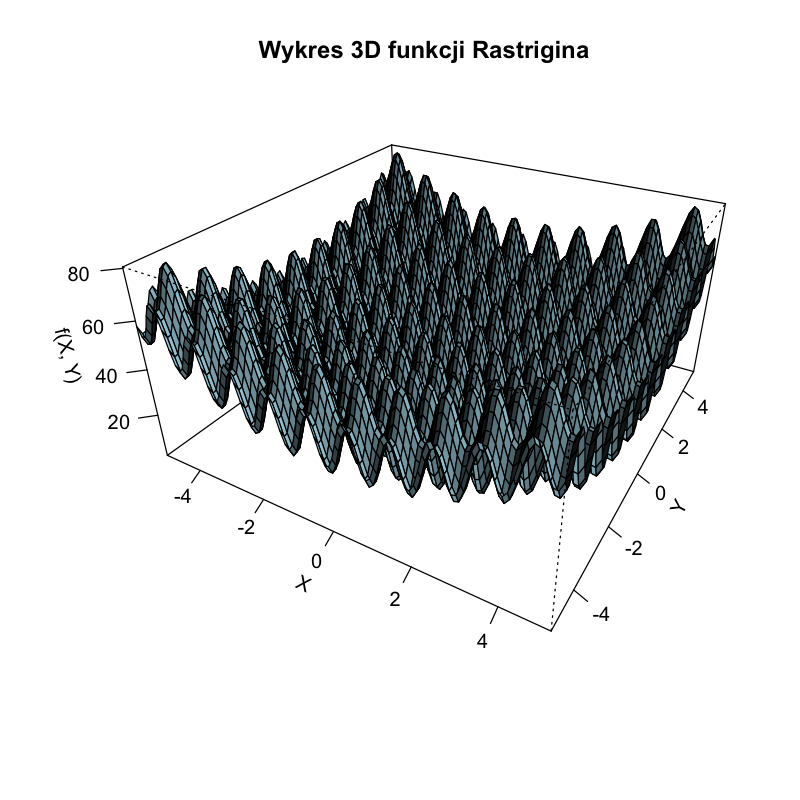
\includegraphics[width=\linewidth]{img/rastrigin_3d.png}
        \caption{Wykres powierzchniowy 3D.}
    \end{minipage}\hfill
    \begin{minipage}{0.48\textwidth}
        \centering
        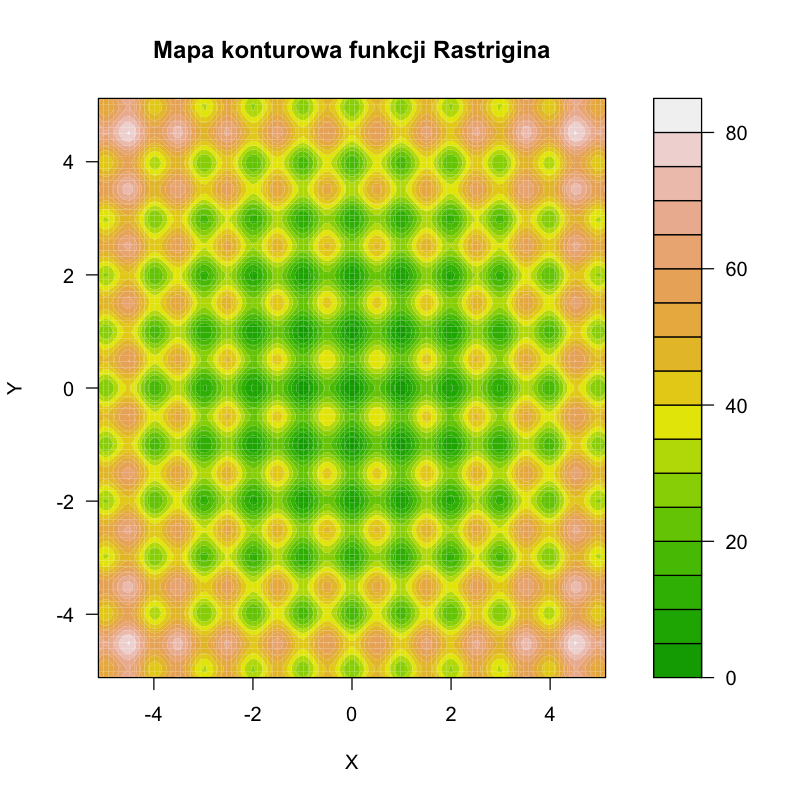
\includegraphics[width=\linewidth]{img/rastrigin_contour.png}
        \caption{Mapa konturowa (widok z góry).}
    \end{minipage}
\end{figure}

\section{Zadanie A: Własne operatory dla algorytmu genetycznego}
Do testów wybrano funkcję Rastrigina, ponieważ jej silnie wielomodalny charakter (rozległa siatka minimów lokalnych) doskonale weryfikuje zdolność nowo zaprojektowanych operatorów do zachowania balansu między globalną eksploracją a lokalną eksploatacją.

\subsection{Szczegółowy opis zaproponowanych operatorów}
Domyślne operatory w bibliotece \texttt{GA} opierają się na selekcji ruletkowej, jednopunktowym krzyżowaniu i mutacji jednorodnej. Zaimplementowano własne funkcje z wykorzystaniem specyfiki przestrzeni ciągłej:

\subsubsection{Własna Selekcja: Turniejowa z progiem (Tournament Selection)}
Zaimplementowano mechanizm \textbf{selekcji turniejowej}. Z populacji losowana jest ze zwracaniem grupa $k=3$ osobników. Do puli rozrodczej przechodzi wyłącznie ten osobnik, którego wartość funkcji przystosowania jest najwyższa. Jest to metoda odporna na problem skalowania i pozwala płynnie sterować presją selekcyjną.

\subsubsection{Własne Krzyżowanie: Uśredniające (Arithmetic Crossover)}
Zamiast krzyżowania punktowego, zaproponowano krzyżowanie oparte na kombinacji liniowej. Potomek powstaje na odcinku łączącym rodziców:
$$x_{potomek} = \alpha \cdot x_{rodzic1} + (1 - \alpha) \cdot x_{rodzic2}$$
gdzie $\alpha \in [0, 1]$ jest losowym współczynnikiem dobieranym dla każdej pary. Pozwala to na precyzyjne odnajdywanie minimów "pomiędzy" już odnalezionymi rozwiązaniami.

\subsubsection{Własna Mutacja: Gaussowska (Gaussian Mutation)}
Wylosowany do mutacji gen $x_i$ jest modyfikowany o losowe zaburzenie:
$$x_i^{nowy} = x_i^{stary} + \mathcal{N}(0, \sigma)$$
gdzie $\mathcal{N}(0, \sigma)$ to wartość z rozkładu normalnego (w badaniach $\sigma = 0.5$). Pozwala to na delikatne dostrajanie rozwiązania z jednoczesną szansą na wyjście z ekstremum lokalnego w przypadku rzadszych, większych zaburzeń.

\subsection{Porównanie wyników}
Przeprowadzono analizę zbieżności algorytmu z wariantem domyślnym oraz z wariantem wykorzystującym zaimplementowane własne operatory (rozmiar populacji = 50, liczba pokoleń = 80).

\begin{figure}[H]
    \centering
    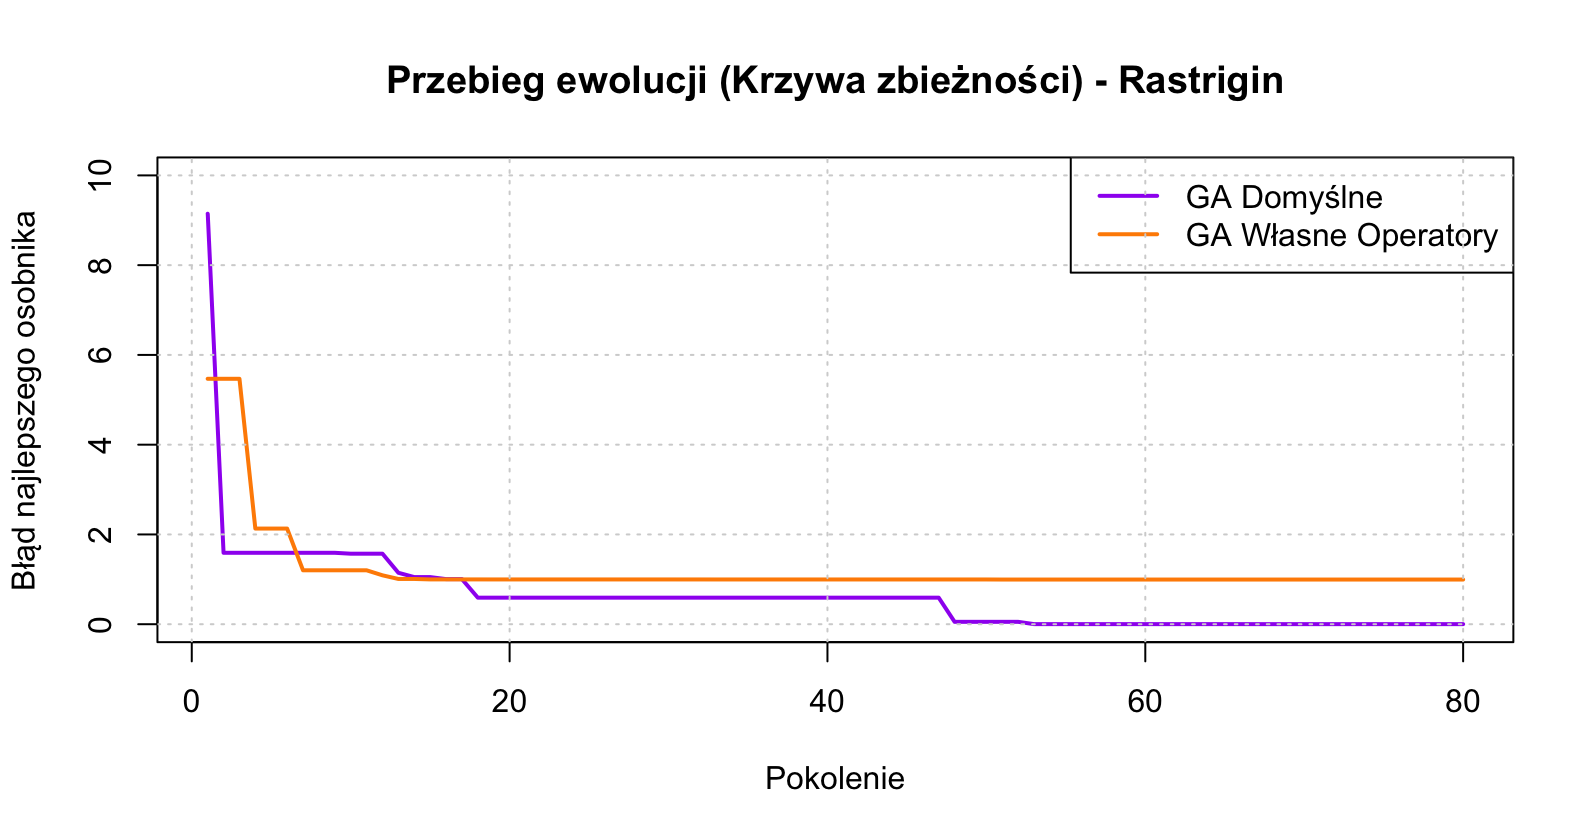
\includegraphics[width=0.8\textwidth]{img/1.png}
    \caption{Przebieg ewolucji (Krzywa zbieżności) - Rastrigin.}
\end{figure}

Krzywa zbieżności jednoznacznie pokazuje, że domyślne operatory pakietu GA poradziły sobie znacznie lepiej. Fioletowa krzywa zbiega niemal idealnie do zera (odnalezienie globalnego minimum). Z kolei wariant z własnymi operatorami (linia pomarańczowa) uległ przedwczesnej zbieżności i utknął na poziomie błędu rzędu $1,0$.

\begin{table}[H]
\centering
\begin{tabular}{lc}
\toprule
\textbf{Wariant Algorytmu} & \textbf{Końcowy błąd (po 80 iteracjach)} \\
\midrule
GA - Operatory Domyślne & $0,0015$ \\
GA - Własne Operatory & $0,9951$ \\
\bottomrule
\end{tabular}
\caption{Porównanie błędu końcowego klasycznego GA i GA z własnymi operatorami.}
\end{table}

\textbf{Wniosek:} Wprowadzenie prostej mutacji Gaussowskiej i krzyżowania arytmetycznego zaburzyło balans eksploracji. Algorytm zaczął zbyt mocno eksploatować lokalne sąsiedztwo, co na silnie wielomodalnej funkcji Rastrigina poskutkowało utknięciem populacji w głębokim minimum lokalnym. Standardowe operatory biblioteki \texttt{GA} posiadają znacznie lepiej zoptymalizowane mechanizmy ucieczki z takich pułapek.

\section{Zadanie D: Badanie algorytmu PSO}
Przeanalizowano wpływ parametrów kontrolnych algorytmu roju cząstek (PSO) minimalizującego funkcję Rastrigina. Wszystkie wyniki przedstawiono jako średni błąd po 10 niezależnych uruchomieniach dla każdego zestawu parametrów.

\subsection{Rozmiar roju ($s$)}
Rozmiar roju warunkuje pokrycie przestrzeni w początkowej fazie działania algorytmu.

\begin{figure}[H]
    \centering
    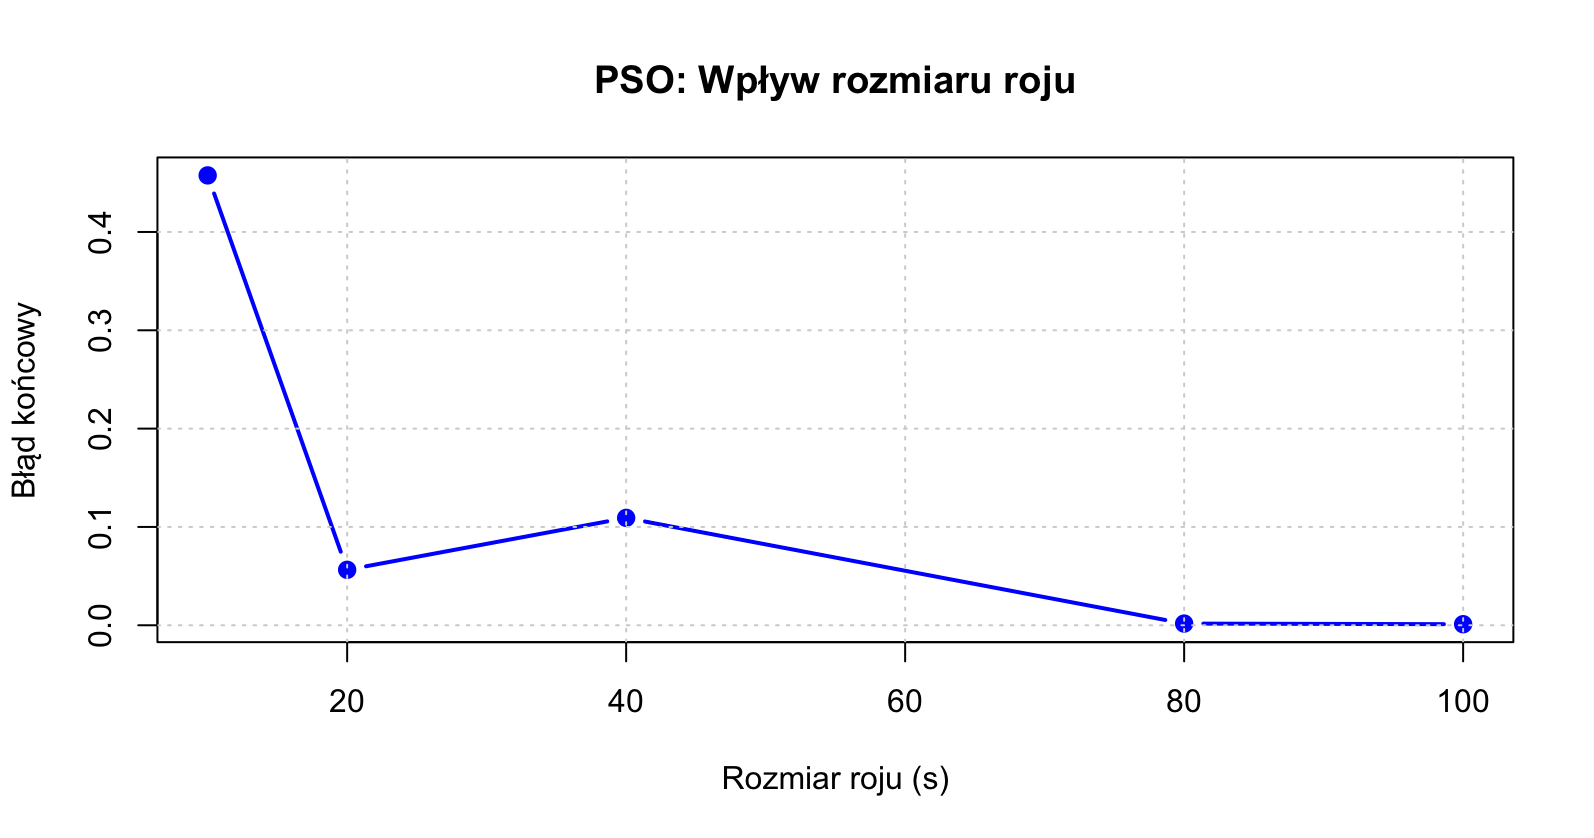
\includegraphics[width=0.8\textwidth]{img/2.png}
    \caption{Wpływ rozmiaru roju na końcowy błąd.}
\end{figure}

Wraz ze wzrostem liczby cząstek, błąd maleje niemal do zera. Ze względu na wielomodalny charakter funkcji, rój poniżej 40 osobników zbyt często wpada w minima lokalne.

\subsection{Współczynnik bezwładności ($w$)}
Parametr ten opisuje skłonność cząstki do zachowania dotychczasowego pędu.

\begin{figure}[H]
    \centering
    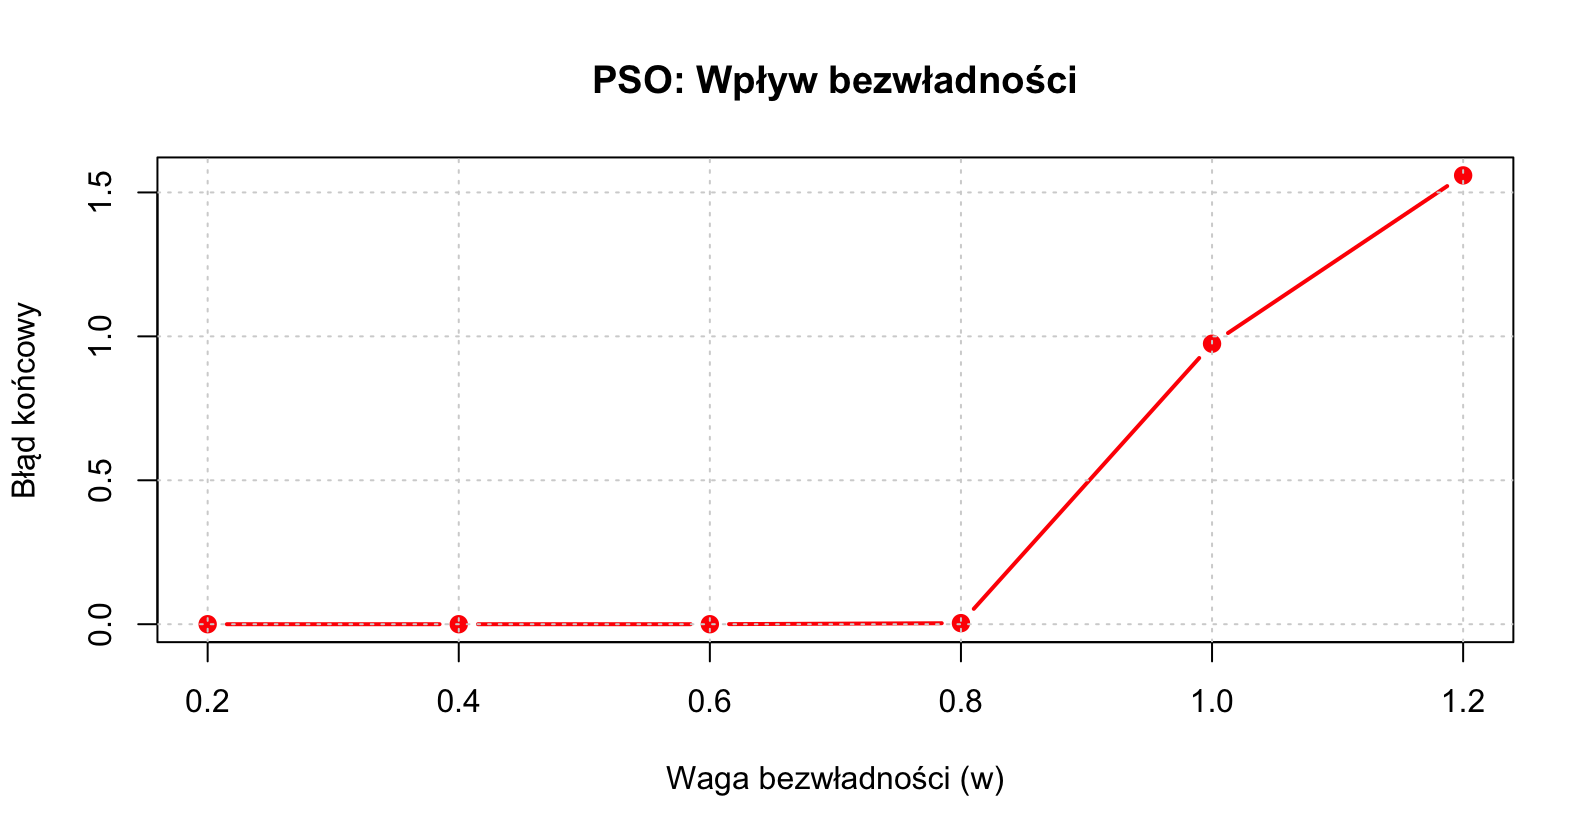
\includegraphics[width=0.7\textwidth]{img/3.png}
    \caption{Wpływ wagi bezwładności na zbieżność.}
\end{figure}

Niska bezwładność ($w \le 0.8$) pozwala rojowi szybko osiadać w ekstremach, gwarantując niskie błędy. Przekroczenie progu $w > 0.8$ skutkuje rozbieganiem się cząstek -- nie są one w stanie wyhamować nad minimum globalnym, co widać jako drastyczny wzrost błędu końcowego.

\subsection{Liczba iteracji (\textit{maxit})}
Zbadano proces uczenia się roju w czasie.

\begin{figure}[H]
    \centering
    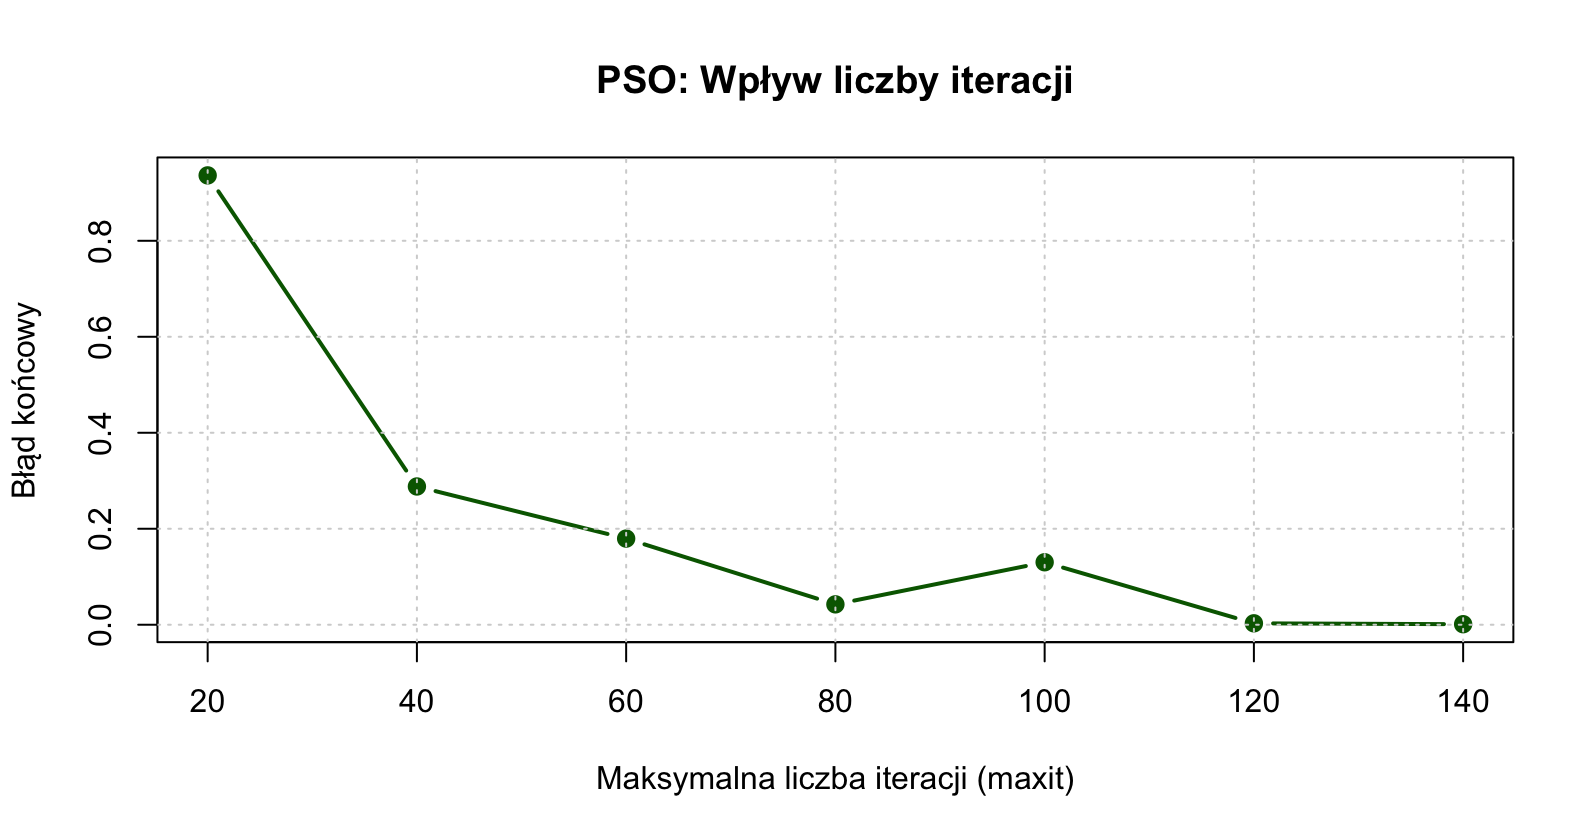
\includegraphics[width=0.7\textwidth]{img/4.png}
    \caption{Krzywa zbieżności PSO w zależności od dostępnych iteracji.}
\end{figure}

Widoczny jest asyptotyczny spadek błędu. Od około 120 iteracji rój w pełni zbiega do globalnego optimum dla uśrednionych parametrów bazowych algorytmu.

\subsection{Współczynniki: kognitywny ($c_p$) i społeczny ($c_g$)}
Współczynnik $c_p$ decyduje o przyciąganiu cząstki do własnej historii, a $c_g$ o zaufaniu do wyników reszty roju.

\begin{figure}[H]
    \centering
    \begin{minipage}{0.48\textwidth}
        \centering
        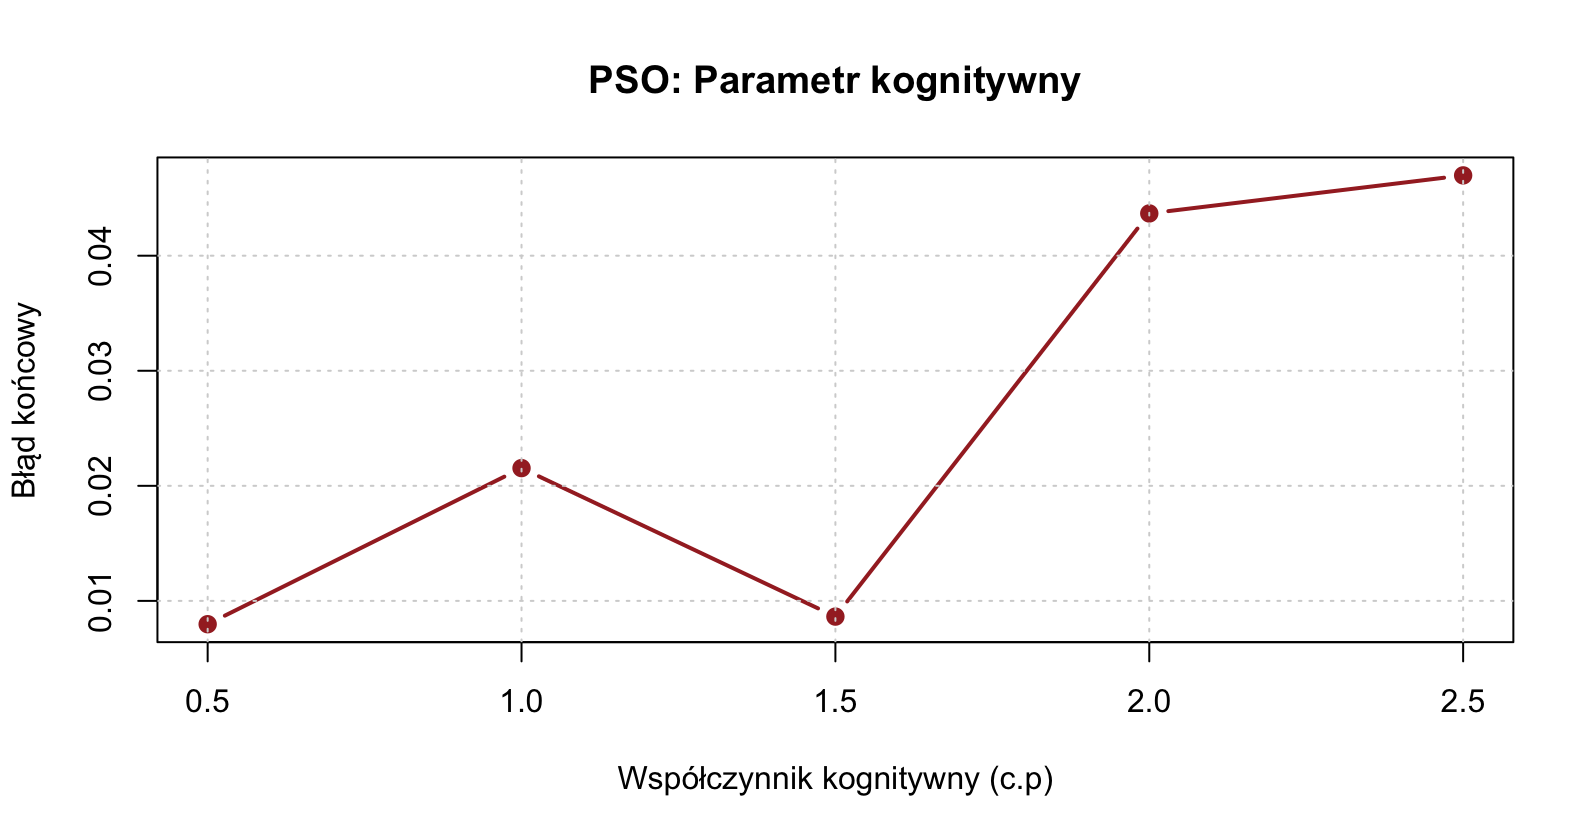
\includegraphics[width=\linewidth]{img/5.png}
        \caption{Wpływ współczynnika kognitywnego.}
    \end{minipage}\hfill
    \begin{minipage}{0.48\textwidth}
        \centering
        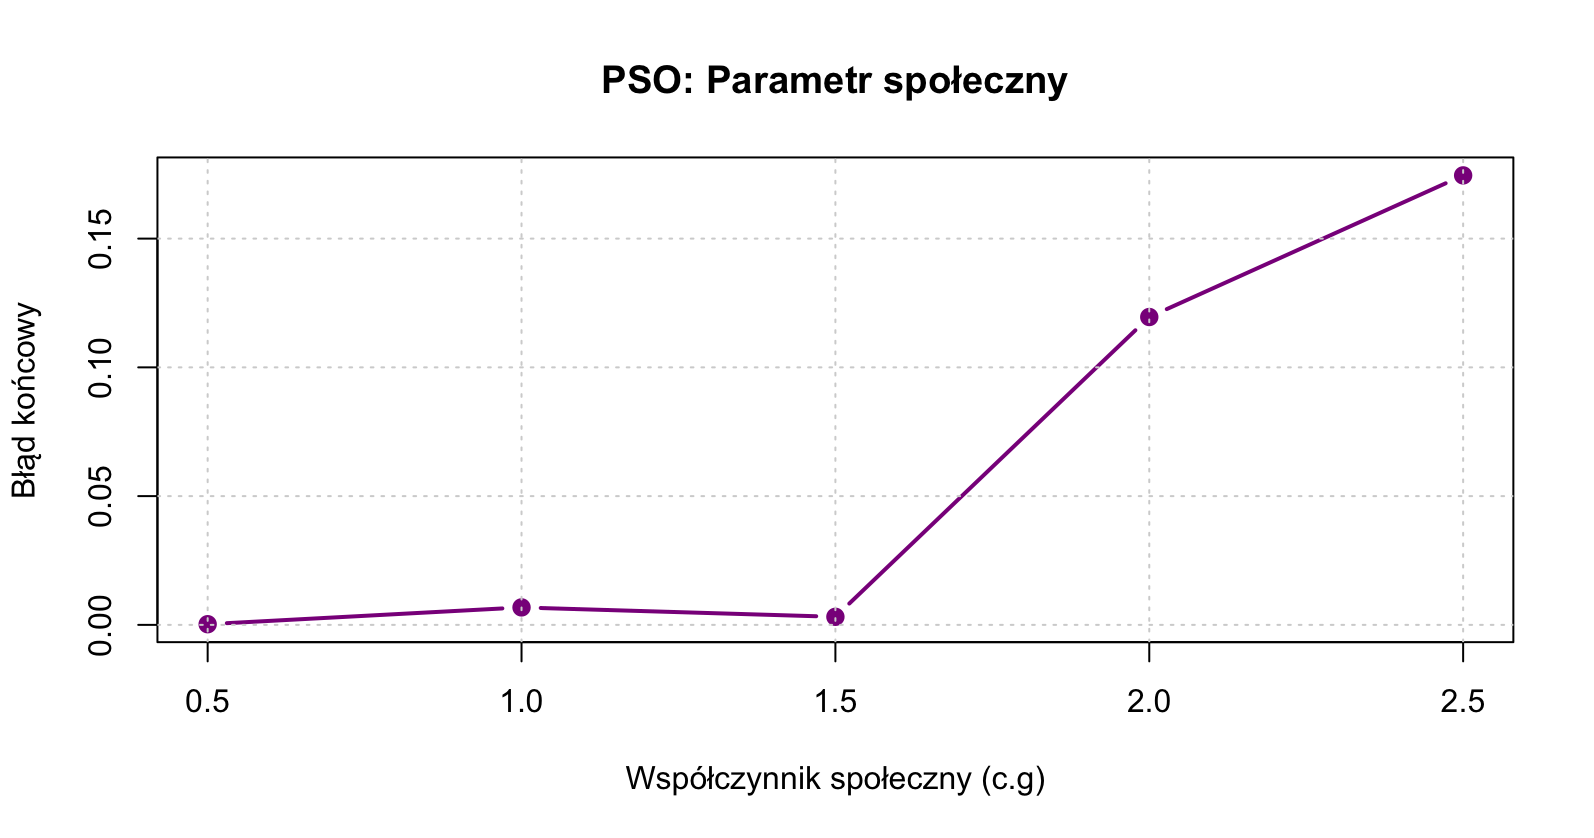
\includegraphics[width=\linewidth]{img/6.png}
        \caption{Wpływ współczynnika społecznego.}
    \end{minipage}
\end{figure}

Zarówno zbyt wysokie zaufanie wyłącznie do własnej pamięci ($c_p > 1.5$), jak i bezgraniczne "śledzenie tłumu" ($c_g > 1.5$) prowadzą do pogorszenia wyników, wybijając algorytm z balansu eksploracyjno-eksploatacyjnego.

\begin{table}[H]
\caption{Szczegółowe dane liczbowe dla badanych parametrów z wygenerowanych wektorów.}
\centering
\begin{tabular}{cc|cc}
\toprule
\textbf{$s$ (Rozmiar roju)} & \textbf{Błąd} & \textbf{ $w$ (Bezwładność)} & \textbf{Błąd} \\
\midrule
10 & $0,4575$ & 0,2 & 0,0000 \\
20 & $0,0564$ & 0,4 & 0,0000 \\
40 & $0,1092$ & 0,6 & 0,0000 \\
80 & $0,0017$ & 0,8 & 0,0037 \\
100 & $0,001$ & 1,0 & 0,9744 \\
-   & -       & 1,2 & 1,5592 \\
\bottomrule
\end{tabular}
\end{table}

\section{Podsumowanie}
Przeprowadzone badania pozwoliły na dogłębną analizę działania algorytmów optymalizacji globalnej na przykładzie silnie wielomodalnej funkcji Rastrigina. Z eksperymentów płyną dwa główne wnioski dotyczące badanych metod.

\textbf{W przypadku Algorytmu Genetycznego (GA)} samodzielna implementacja operatorów (krzyżowanie arytmetyczne, mutacja Gaussowska) wykazała, jak delikatny jest balans między eksploracją (przeszukiwaniem nowych obszarów) a eksploatacją (zawężaniem poszukiwań). Zastosowane własne metody doprowadziły do przedwczesnej zbieżności i utknięcia populacji w minimum lokalnym. Stanowi to dowód na to, że domyślne operatory wbudowane w pakiety optymalizacyjne są wysoce dopracowane i znacznie skuteczniej radzą sobie z ucieczką z pułapek lokalnych ekstremów.

\textbf{W przypadku Optymalizacji Rojem Cząstek (PSO)} algorytm ten okazał się niezwykle skuteczny, ale jednocześnie wrażliwy na dobór parametrów kontrolnych. Kształt funkcji Rastrigina wymusza zastosowanie relatywnie dużej populacji początkowej ($s \ge 40$), aby od samego początku dobrze pokryć przestrzeń poszukiwań. Kluczowym parametrem okazała się waga bezwładności ($w$) -- jej optymalna wartość w okolicach $0.8$ pozwala na płynne zbieganie roju. Nawet niewielkie odchylenia od tej wartości skutkują zjawiskiem rozbiegania się cząstek lub natychmiastowym utknięciem w pierwszym napotkanym minimum lokalnym.

Ostatecznie można stwierdzić, że optymalizacja funkcji ciągłych o tak skomplikowanej topologii wymaga nie tylko doboru odpowiedniego algorytmu, ale także świadomego procesu strojenia jego parametrów.

\renewcommand{\refname}{Literatura}
\begin{thebibliography}{9}

\bibitem{ga_package}
Scrucca L. (2013). \textit{GA: A Package for Genetic Algorithms in R}. Journal of Statistical Software, 53(4), 1-37.

\bibitem{pso_package}
Bendtsen C. (2012). \textit{pso: Particle Swarm Optimization}. R package version 1.0.3.

\bibitem{pso_theory}
Kennedy, J., \& Eberhart, R. (1995). \textit{Particle swarm optimization}. Proceedings of ICNN'95 - International Conference on Neural Networks, vol. 4, 1942-1948.

\end{thebibliography}

\newpage
\appendix
\section{Załącznik: Kod źródłowy w języku R}
Poniżej znajduje się kompletny skrypt wykorzystany do generowania wyników i wykresów.

\begin{lstlisting}[language=R]
library(GA)
library(pso)
set.seed(42)

# --- 1. FUNKCJE BAZOWE ---
rastrigin <- function(x1, x2) { 20 + (x1^2 - 10 * cos(2 * pi * x1)) + (x2^2 - 10 * cos(2 * pi * x2)) }
fit_ga <- function(x) { -rastrigin(x[1], x[2]) }
fit_pso <- function(x) { rastrigin(x[1], x[2]) }

# --- 2. WLASNE OPERATORY GA ---
custom_tourSel <- function(obj, k=3) {
  pop <- obj@population; fit <- obj@fitness; sel <- rep(NA, obj@popSize)
  for(i in 1:obj@popSize) { sel[i] <- sample(1:obj@popSize, k)[which.max(fit[sample(1:obj@popSize, k)])] }
  list(population = pop[sel,,drop=FALSE], fitness = fit[sel])
}
custom_arithCross <- function(obj, par) {
  p1 <- obj@population[par[1],]; p2 <- obj@population[par[2],]; a <- runif(1)
  list(children = rbind(a*p1 + (1-a)*p2, (1-a)*p1 + a*p2), fitness = c(NA, NA))
}
custom_gaussMut <- function(obj, par) {
  m <- as.vector(obj@population[par,]); j <- sample(1:length(m), 1)
  m[j] <- min(max(m[j] + rnorm(1, 0, 0.5), obj@lower[j]), obj@upper[j]); m
}

# --- 3. KRZYWA ZBIEZNOSCI GA (Domyslne vs Wlasne) ---
cat("Generowanie krzywej zbieznosci GA...\n")
ga_default <- ga(type="real-valued", fitness=fit_ga, lower=c(-5.12,-5.12), upper=c(5.12,5.12), popSize=50, maxiter=80, monitor=FALSE)
ga_custom <- ga(type="real-valued", fitness=fit_ga, lower=c(-5.12,-5.12), upper=c(5.12,5.12), popSize=50, maxiter=80, 
                selection=custom_tourSel, crossover=custom_arithCross, mutation=custom_gaussMut, monitor=FALSE)

plot(1:80, -ga_default@summary[, "max"], type="l", lwd=2, col="purple", ylim=c(0, 10),
     main="Przebieg ewolucji (Krzywa zbieznosci) - Rastrigin", xlab="Pokolenie", ylab="Blad najlepszego osobnika")
lines(1:80, -ga_custom@summary[, "max"], lwd=2, col="darkorange")
legend("topright", legend=c("GA Domyslne", "GA Wlasne Operatory"), col=c("purple", "darkorange"), lwd=2)
grid()

# --- 4. FUNKCJA TESTUJACA PSO ---
run_pso <- function(s=40, maxit=100, w=0.8, cp=1.5, cg=1.5) {
  mean(sapply(1:10, function(i) {
    psoptim(runif(2, -5.12, 5.12), fit_pso, lower=c(-5.12,-5.12), upper=c(5.12,5.12), 
            control=list(s=s, maxit=maxit, w=w, c.p=cp, c.g=cg))$value
  }))
}

cat("Obliczanie parametrow PSO...\n")

# Wykres 1: Rozmiar roju
v_s <- c(10, 20, 40, 80, 100); r_s <- sapply(v_s, function(x) run_pso(s=x))
plot(v_s, r_s, type="b", pch=19, col="blue", lwd=2, main="PSO: Wplyw rozmiaru roju", xlab="Rozmiar roju (s)", ylab="Blad koncowy"); grid()

# Wykres 2: Bezwladnosc
v_w <- seq(0.2, 1.2, by=0.2); r_w <- sapply(v_w, function(x) run_pso(w=x))
plot(v_w, r_w, type="b", pch=19, col="red", lwd=2, main="PSO: Wplyw bezwladnosci", xlab="Waga bezwladnosci (w)", ylab="Blad koncowy"); grid()

# Wykres 3: Liczba iteracji
v_i <- c(20, 40, 60, 80, 100, 120, 140); r_i <- sapply(v_i, function(x) run_pso(maxit=x))
plot(v_i, r_i, type="b", pch=19, col="darkgreen", lwd=2, main="PSO: Wplyw liczby iteracji", xlab="Maksymalna liczba iteracji (maxit)", ylab="Blad koncowy"); grid()

# Wykres 4: Parametr kognitywny (c.p)
v_cp <- seq(0.5, 2.5, by=0.5); r_cp <- sapply(v_cp, function(x) run_pso(cp=x))
plot(v_cp, r_cp, type="b", pch=19, col="brown", lwd=2, main="PSO: Parametr kognitywny", xlab="Wspolczynnik kognitywny (c.p)", ylab="Blad koncowy"); grid()

# Wykres 5: Parametr spoleczny (c.g)
v_cg <- seq(0.5, 2.5, by=0.5); r_cg <- sapply(v_cg, function(x) run_pso(cg=x))
plot(v_cg, r_cg, type="b", pch=19, col="darkmagenta", lwd=2, main="PSO: Parametr spoleczny", xlab="Wspolczynnik spoleczny (c.g)", ylab="Blad koncowy"); grid()
\end{lstlisting}

\end{document}